\documentclass[UTF8]{ctexart}
\usepackage{CJKutf8}
\usepackage{graphicx}
\usepackage{amsmath}
\usepackage{xcolor}
\usepackage{cite}
\usepackage{amssymb}
\usepackage{indentfirst}
\usepackage{hyperref}
  \author{黄晃 数院 1701210098 }
  \title{有限元上机作业}
\begin{document}
  \maketitle
\section{问题}
求解在平面应变或平面应力假设下的二维弹性力学问题
\begin{itemize}
  \item 计算区域为10cm$\times10cm$的正方形
  \item 边界条件:下边界固定,其余三边自由.
  \item 受力情况:左上角受到大小为f,方向为$\frac{3}{2}\pi$的力
  \item 参数:$\lambda=3.65\times 10^4Mpa,\lambda+2\mu = 6.70\times 10^4Mpa$
\end{itemize}
\subsection{弹性力学方程}
位移为$\mathbf{u}=[u,v,w]^T \in\mathbb{R}^3$,应力$\sigma \in S^{3\times 3}$,应变$\epsilon\in S^{3\times3}$
满足:
\begin{itemize}
  \item 平衡方程
  $$
  -div(\sigma)=g
  $$
  \item 几何方程
  $$
  \epsilon = \frac{1}{2}(\nabla \mathbf{u} + \nabla \mathbf{u}^T)
  $$
  \item 本构方程
  $$
  \sigma = 2\mu \epsilon + \lambda tr(\epsilon)I
  $$
  \item 消去应力应变,得:
  $$
  -\mu \triangle \mathbf{u} - (\lambda+\mu)\nabla(\nabla\mathbf{u})=g,\ \mathbf{x}\in \Omega
  $$
  边界条件
  \begin{align*}
  \sum_{j=1}^{3}\sigma_{ij}n_j = f_i & ,\ \mathbf{x}\in \Gamma_1 \\
    \mathbf{u}=0 & ,\ \mathbf{x}\in \Gamma_0
  \end{align*}
\end{itemize}
\subsection{二维弹性力学问题}
选择平面应变假设:
$$
u = u(x,y),v=v(x,y),w=0
$$
则有
$$
u_z = v_z=0,w_x=w_y=w_z=0
$$
我们将方程写成分量形式
\begin{equation}\label{p0}
  -\mu\left[
  \begin{matrix}
    u_{xx} + u_{yy} \\
     v_{xx} + v_{yy}
  \end{matrix}
  \right]
-(\lambda+\mu]\left[
  \begin{matrix}
    u_{xx} + v_{xy} \\
     u_{xy} + v_{yy}
  \end{matrix}
  \right]
=
  \left[
  \begin{matrix}
    g_x \\
     g_y
  \end{matrix}
  \right]
  \end{equation}
其中$g_x,g_y$分别是体力$g$在x,y方向上的分量.由于$w=0$,之后我们记$\mathbf{u}=[u,v]\in \mathbb{R}^2$
\subsection{变分问题}
在方程~\ref{p0}两端同乘检验函数$\mathbf{v}=[p,q]\in \mathbb{R}^2,\mathbf{v}|_{\Gamma_0}=0$,有
$$
-\mu (\triangle u p + \triangle v q) -\mu(div(\mathbf{u}_x)p+div(\mathbf{u}_y)q) -\lambda (div([u_x+v_y,0])p+div([0,u_x+v_y])q)  = g_xp+g_yq.
$$
在$\Omega$上积分,由Green公式,有
\begin{align*}
  \int_{\Omega}-\mu (\triangle u p + \triangle v q)d\mathbf{x} & =\int_{\Gamma}-\mu (\nabla u p\cdot n+\nabla v q\cdot n) ds + \int_{\Omega}\mu (\nabla u \nabla p+\nabla v \nabla q)d\mathbf{x}  \\
  \int_{\Omega}-\mu(div(\mathbf{u}_x)p+div(\mathbf{u}_y)q) & =\int_{\Gamma} -\mu(\mathbf{u}_x p\cdot n+\mathbf{u}_y q\cdot n) ds + \int_{\Omega}\mu(\mathbf{u}_x \nabla p+\mathbf{u}_y \nabla q)d\mathbf{x} \\
\int_{\Omega}-\lambda(div([u_x+v_y,0])p+div([0,u_x+v_y])q) &=\int_{\Gamma} -\lambda ([u_x+v_y,0] p\cdot n+[0,u_x+v_y] q\cdot n) ds \\
  &+ \int_{\Omega}\lambda([u_x+v_y,0] \nabla p+[0,u_x+v_y] \nabla q)d\mathbf{x}
\end{align*}
而
\begin{align*}
 & \ \int_{\Gamma}-\mu (\nabla u p\cdot n+\nabla v q\cdot n) ds -\int_{\Gamma} \mu(\mathbf{u}_x p\cdot n+\mathbf{u}_y q\cdot n) ds   -\int_{\Gamma} \lambda ([u_x+v_y,0] p\cdot n+[0,u_x+v_y] q\cdot n) ds\\
   & =\int_{\Gamma} ((-\mu(\nabla u+ \mathbf{u}_x)-\lambda[u_x+v_y,0] )p+((-\mu(\nabla v + \mathbf{u}_y))-\lambda[0,u_x+v_y] )q) \cdot n ds \\
 & =\int_{\Gamma} p(-\mu(\nabla u+\mathbf{u}_x)-\lambda [u_x+v_y,0] )\cdot n ds+\int_{\Gamma}q(-\mu(\nabla v+\mathbf{u}_y))-\lambda[0,u_x+v_y] ) \cdot n ds \\
&= -\int_{\Gamma}p[\sigma_{11},\sigma_{12}]\cdot n ds - \int_{\Gamma}q[\sigma_{21},\sigma_{22}]\cdot n ds
\end{align*}
由边界条件,我们有
\begin{align*}
  p,q & =0,\ \mathbf{x} \in \Gamma_0 \\
  \sum_{i=1}^{2}\sigma_{1i}n_i  & =f_j  ,\ \mathbf{x} \in \Gamma_1
\end{align*}
所以有
$$
-\int_{\Gamma}p[\sigma_{11},\sigma_{12}]\cdot n ds - \int_{\Gamma}q[\sigma_{21},\sigma_{22}]\cdot n ds =
-\int_{\Gamma_1}pf_1 +qf_2ds
$$
因此,我们有了弱形式:
\begin{equation}\label{p1}
a(\mathbf{u},\mathbf{v}) = F(\mathbf{v})
\end{equation}
其中
\begin{align*}
a(\mathbf{u},\mathbf{v}) & = \int_{\Omega}\mu (\nabla u \nabla p+\nabla v \nabla q)d\mathbf{x}  +   \int_{\Omega}\mu(\mathbf{u}_x \nabla p+\mathbf{u}_y \nabla q)d\mathbf{x} + \int_{\Omega}\lambda([u_x+v_y,0] \nabla p+[0,u_x+v_y] \nabla q)d\mathbf{x} \\
 &=            \\
F(\mathbf{v}) &= \int_{\Gamma_1}pf_1 +qf_2ds +\int_{\Omega}g_xp+g_yqd\mathbf{x}
\end{align*}
\section{有限元方法}
对于上面的变分问题,选择三角形P1元有限元方法求解.
\subsection{网格}
对区域$\Omega$做三角形剖分,两个方向n等分,共$(n+1)^2$个节点,$2n^2$个单元.单元编号以及点编号都以行优先的顺序.n=3时网格如图~\ref{grid}
\begin{figure}[htbp]
\centering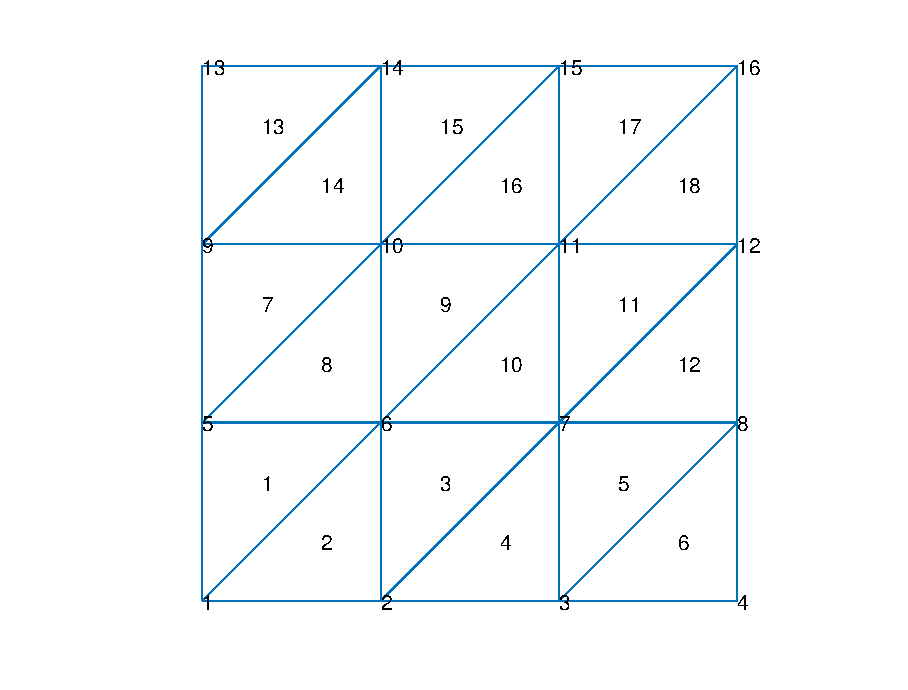
\includegraphics[width=3.5in]{gird.eps}
\caption{grid}\label{grid}
\end{figure}
\subsection{自由度和基函数}
由于我们的解空间为$V=\{ v \in (H^1(\Omega)) ^2 :\  v|_{\Gamma_0}=0\}$,所以在每个单元上有6个自由度:
$$
\Sigma_K = \{u(a_i),v(a_i):i=1,2,3\}
$$
对应的基函数为
\begin{equation}
\phi_1 = \left[
    \begin{matrix}
    \lambda_1(x,y) \\
     0
  \end{matrix}\right]
  ,\ \phi_2 = \left[
      \begin{matrix}
    \lambda_2(x,y) \\
     0
  \end{matrix}\right]
  ,\ \phi_3 = \left[
      \begin{matrix}
    \lambda_3(x,y) \\
     0
  \end{matrix} \right]
  ,\ \phi_4 = \left[
      \begin{matrix}
    0 \\
     \lambda_1(x,y)
  \end{matrix} \right]
  ,\ \phi_5 = \left[
        \begin{matrix}
    0 \\
     \lambda_2(x,y)
  \end{matrix}
 \right]
  ,\ \phi_6 = \left[
        \begin{matrix}
    0 \\
     \lambda_3(x,y)
  \end{matrix}
 \right]
\end{equation}

因为双线性函数$a(\mathbf{u},\mathbf{v})$只有导数项,所以坐标系平移没影响,下面假定在每个单元上左下角节点为(0,,0),逆时针给节点编号,则质心坐标为:
\begin{equation}
  \left\{
  \begin{array}{cccc}
    \lambda_1 = 1-\frac{y}{h}, &\lambda_2=\frac{x}{h}  &\lambda_3 = \frac{y}{h}-\frac{x}{h}  & 2\nmid k  \\
   \lambda_1 = 1-\frac{x}{h}, &\lambda_2=\frac{x}{h}-\frac{y}{h}  &\lambda_3 = \frac{y}{h}  & 2 | n
  \end{array}
  \right.
\end{equation}
\subsection{单刚}
由于是规则网格,所以我们不借助参考单元,直接在单元K上计算单刚系数$a(\phi_i,\phi_j)$,
\begin{itemize}
  \item 奇数单元上单刚为
  \begin{equation}\notag
    \frac{1}{2} \left[
    \begin{matrix}
      \mu & 0 & -\mu & 0& -\mu &\mu \\
      0 & \lambda + 2\mu & -\lambda-2\mu & -\lambda & 0 & \lambda \\
      -\mu & -\lambda-2\mu & \lambda+3\mu & \lambda & \mu & -\lambda-\mu \\
      0 & -\lambda & \lambda & \lambda + 2\mu & 0 & -\lambda-2\mu \\
      -\mu & 0 & \mu & 0 & \mu & -\mu\\
      \mu & \lambda & -\lambda-\mu & -\lambda-2\mu & -\mu &\lambda+3\mu
    \end{matrix}
    \right]
  \end{equation}
  \item 偶数单元上单刚为
    \begin{equation}\notag
    \frac{1}{2} \left[
    \begin{matrix}
      \lambda+2\mu & -\lambda-2\mu &0 & 0& \lambda &-\lambda \\
      -\lambda-2\mu & \lambda + 3\mu & -\mu & \mu & -\lambda-\mu & \lambda \\
      0 & -\mu & \mu & -\mu& \mu &0 \\
      0 & \mu & -\mu  & \mu & -\mu  & 0 \\
      \lambda & -\lambda-\mu & \mu & -\mu & \lambda + 3\mu &-\lambda-2\mu\\
      -\lambda & \lambda & 0 & 0 & -\lambda-2\mu &\lambda+2\mu
    \end{matrix}
    \right]
  \end{equation}
\end{itemize}
\subsection{刚度矩阵}
整体刚度矩阵的形成可以先将每个单元的单刚相加,然后将强制边界条件上的节点所在行,列除对角元全部置0即可.
\subsection{右端项}
首先该问题中体力项g=0,所以右端项只剩下$\int_{\Gamma_1}pf_1 +qf_2ds$.我们将问题所给的集中力处理为只在左上单元处起作用的面力.则除了该单元(2n(n-1)+1),其余单元对应的右端项均为0.而该单元上产生的右端项为
\begin{equation}\notag
  F(i) = \left\{
  \begin{array}{cc}
    \frac{\sqrt{2}}{4}hf, & i=en(1,2n(n-1)+1),en(3,2n(n-1)+1) \\
    -\frac{\sqrt{2}}{4}hf, & i=en(5,2n(n-1)+1),en(6,2n(n-1)+1)
  \end{array}
  \right.  
\end{equation}
其中en(i,k)为第k个单元上第i个节点在整体的编号.
\section{计算结果}
下面给出n=100,f=10时的计算结果.由于采用的应变假设,所以z方向应力计算公式为:
$$
\sigma_z = \lambda tr(\epsilon)
$$
\begin{figure}[htbp]
\centering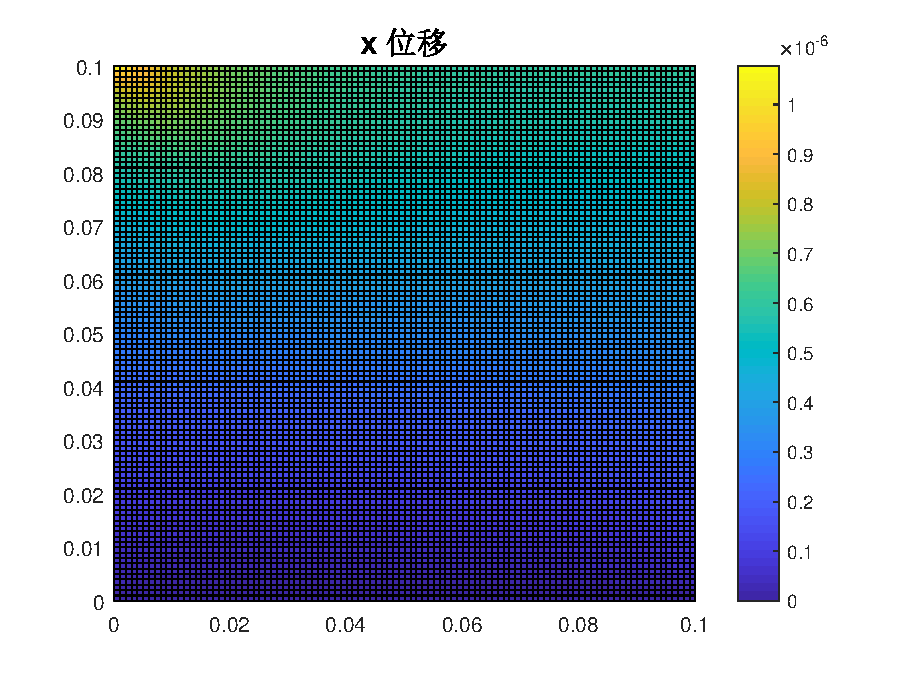
\includegraphics[width=3.5in]{dispx.eps}

\end{figure}
\begin{figure}[htbp]
\centering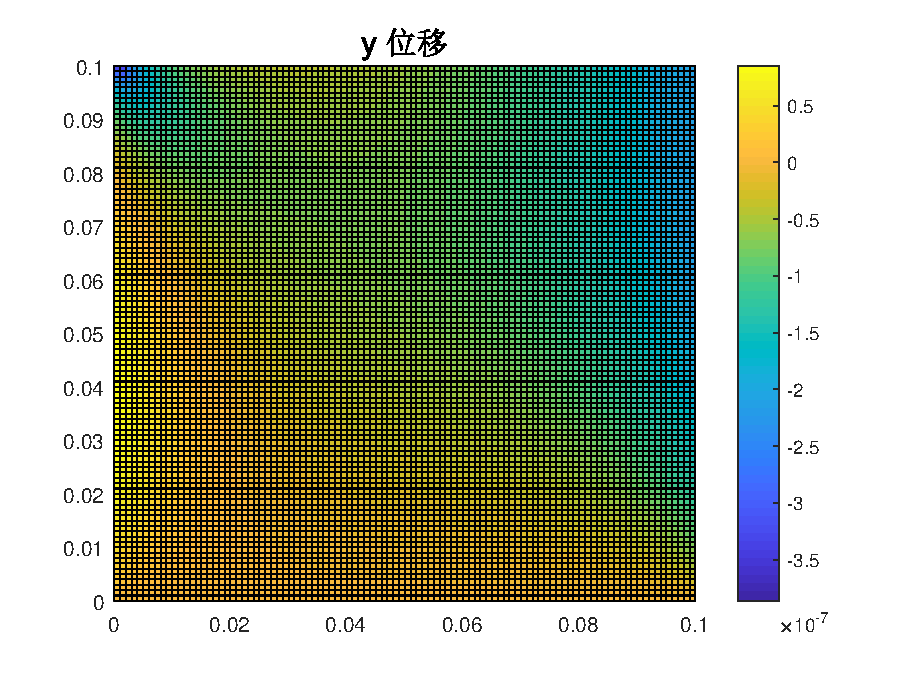
\includegraphics[width=3.5in]{dispy.eps}

\end{figure}
\begin{figure}[htbp]
\centering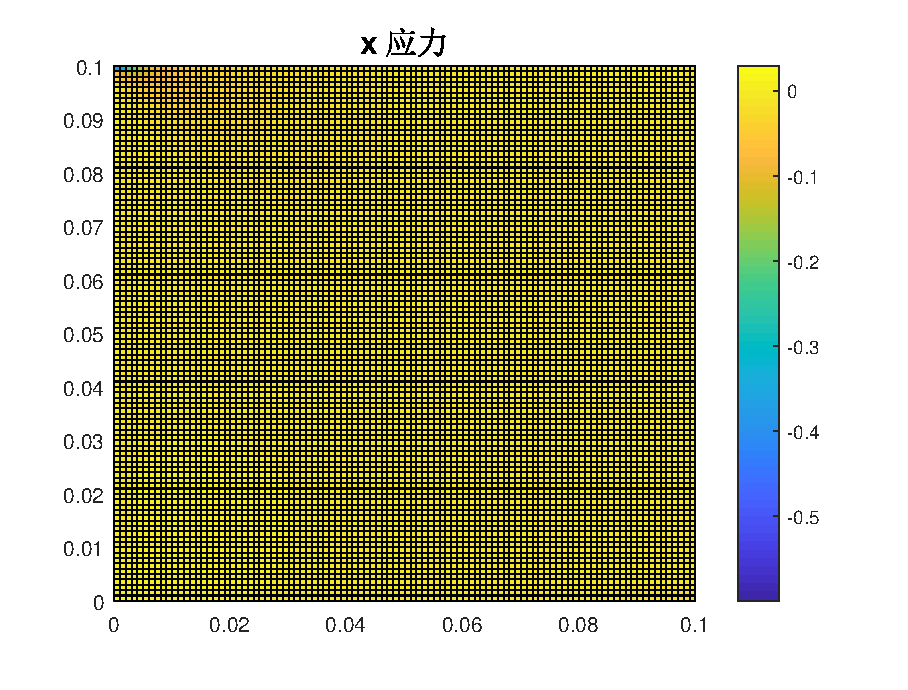
\includegraphics[width=3.5in]{stressx.eps}

\end{figure}
\begin{figure}[htbp]
\centering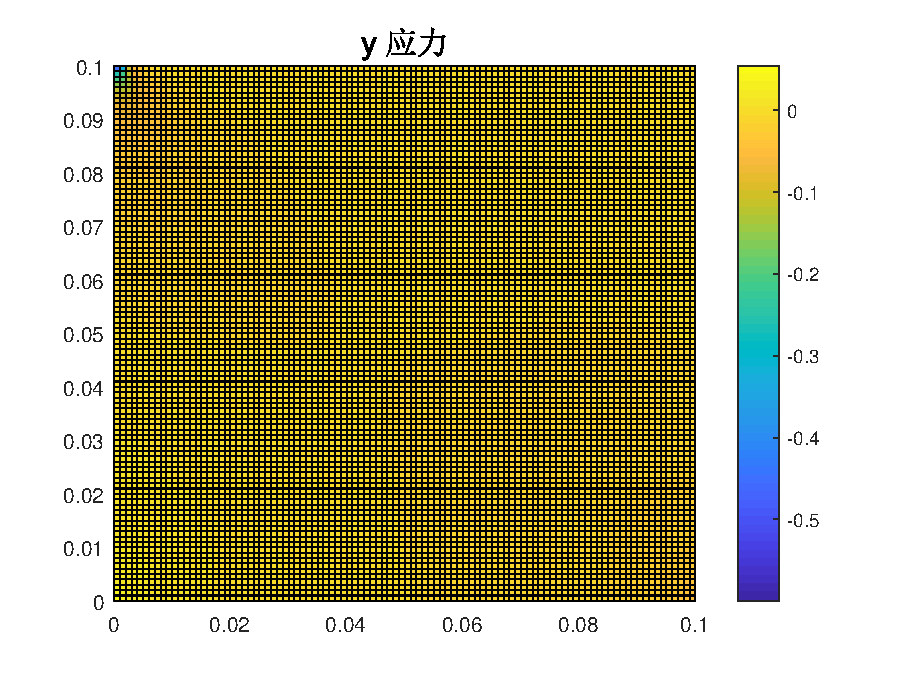
\includegraphics[width=3.5in]{stressy.eps}

\end{figure}
\begin{figure}[htbp]
\centering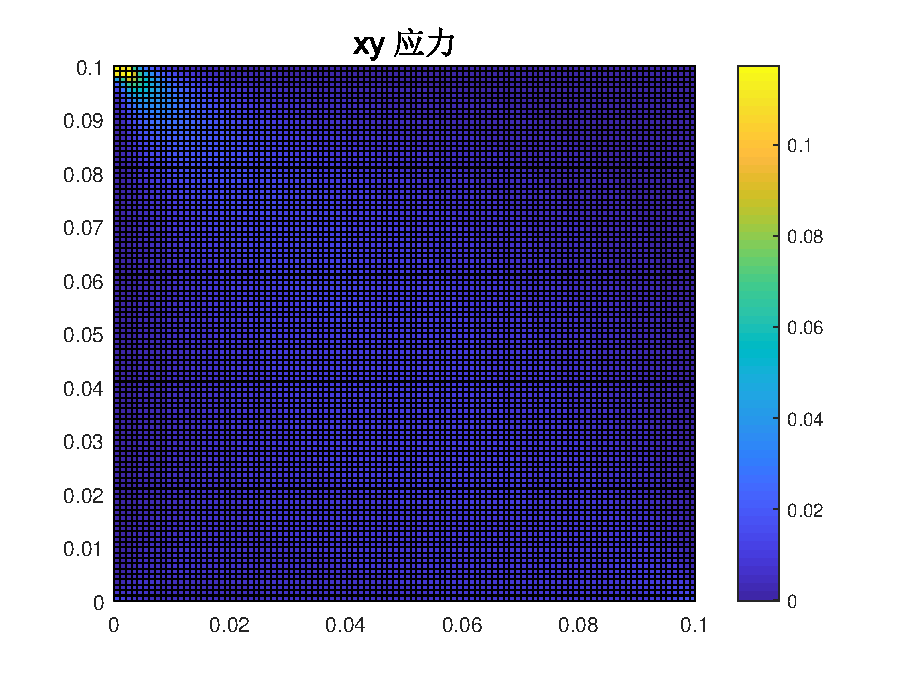
\includegraphics[width=3.5in]{stressxy.eps}

\end{figure}
\begin{figure}[htbp]
\centering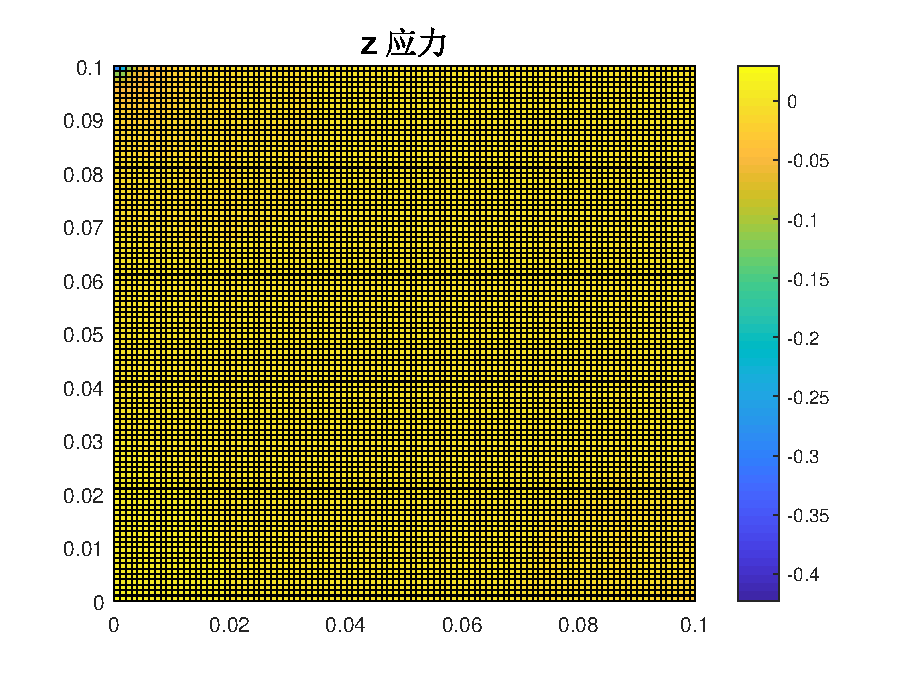
\includegraphics[width=3.5in]{stressz.eps}

\end{figure}
\end{document}
